\section{Advanced architecture development}
In questa sezione viene analizzato il progetto dello stesso filtro IIR visto in precedenza ma con un'architettura avanzata, sviluppata con la tecnica del J-look-ahead. L'equazione di base del filtro è la seguente:
$$ y[n] = b_0x[n] + b_1x[n-1] + a_1y[n-1]$$

La tecnica del J-look-ahead prevede di riscrivere l'equazione andando a sostituire il termine $y[n-1]$ valutandolo in funzione di $y[n-2]$. 
$$ y[n-1] = b_0x[n-1] + b_1x[n-2] + a_1y[n-2]$$

Quindi è possibile sostituire nell'equazione di partenza il risultato ottenuto:
$$ y[n] = b_0x[n] + b_1x[n-1] + a_1(b_0x[n-1] + b_1x[n-2] + a_1y[n-2])$$
$$ y[n] = b_0x[n] + (b_1 + a_1)x[n-1] + a_1b_1x[n-2] + {a_1}^{2}y[n-2]$$

Mantenendo l'architettura classica del filtro IIR direct form II, si nota che l'equazione risultante può essere implementata attraverso lo schema di un filtro di secondo ordine. 

\begin{figure}[h]
	\center
	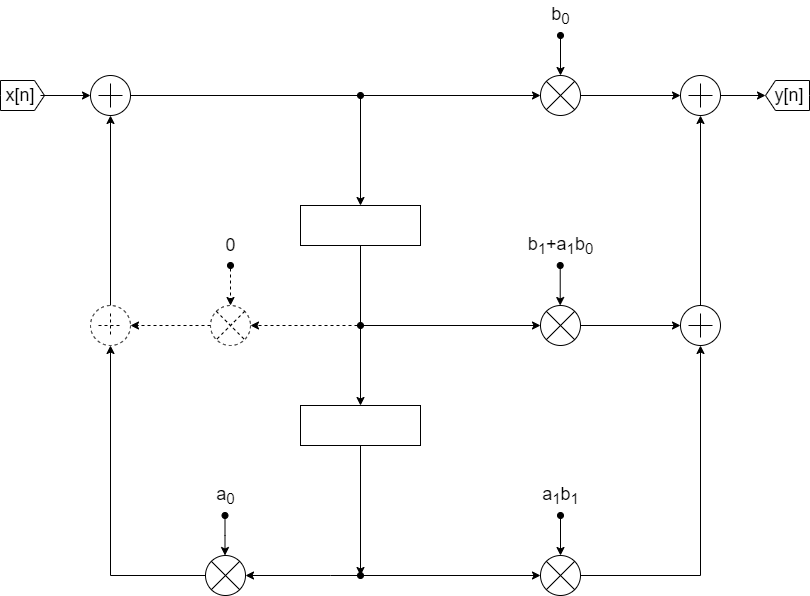
\includegraphics[width=0.7\textwidth]{IIR_2.png}
	\caption{IIR filter with J-look-ahead technique}
	\label{fig:IIR_advanced}
\end{figure}

Questa struttura può essere, al contrario di quella precedente, migliorata in termini di prestazioni. Il percorso critico di questo schema è composto da 4 blocchi combinatori, due moltiplicatori e due sommatori ma attraverso le opportune trasformazioni è possibile ridurre il percorso combinatorio più lungo. In \autoref{fig:IIR_advanced_2} è stato identificato il primo cut-set che permette di spostare il registro modificando la lunghezza del percorso critico portandola da 4 a 3.

\begin{figure}[h]
	\center
	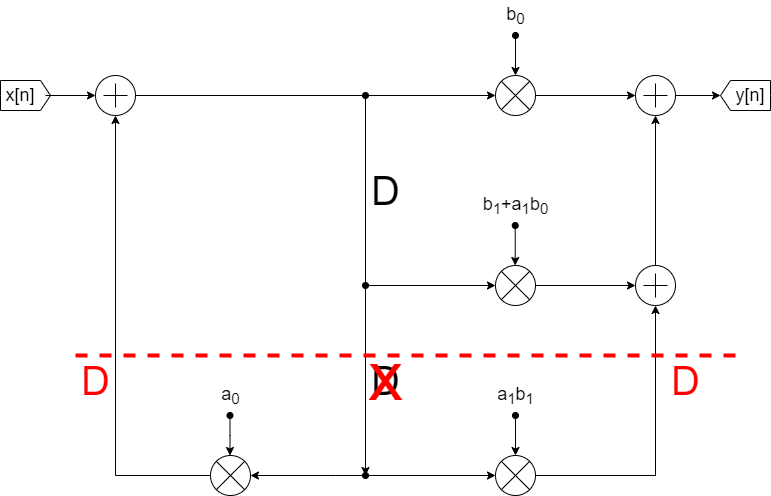
\includegraphics[width=0.7\textwidth]{IIR_2_1.png}
	\caption{Advanced architecture with $1^{st}$ transformation}
	\label{fig:IIR_advanced_2}
\end{figure}

